\begin{figure}[ht]
\centering
% \vspace{0.2em} % 增加上方空白
% \hspace{1em} % 增加左方空白
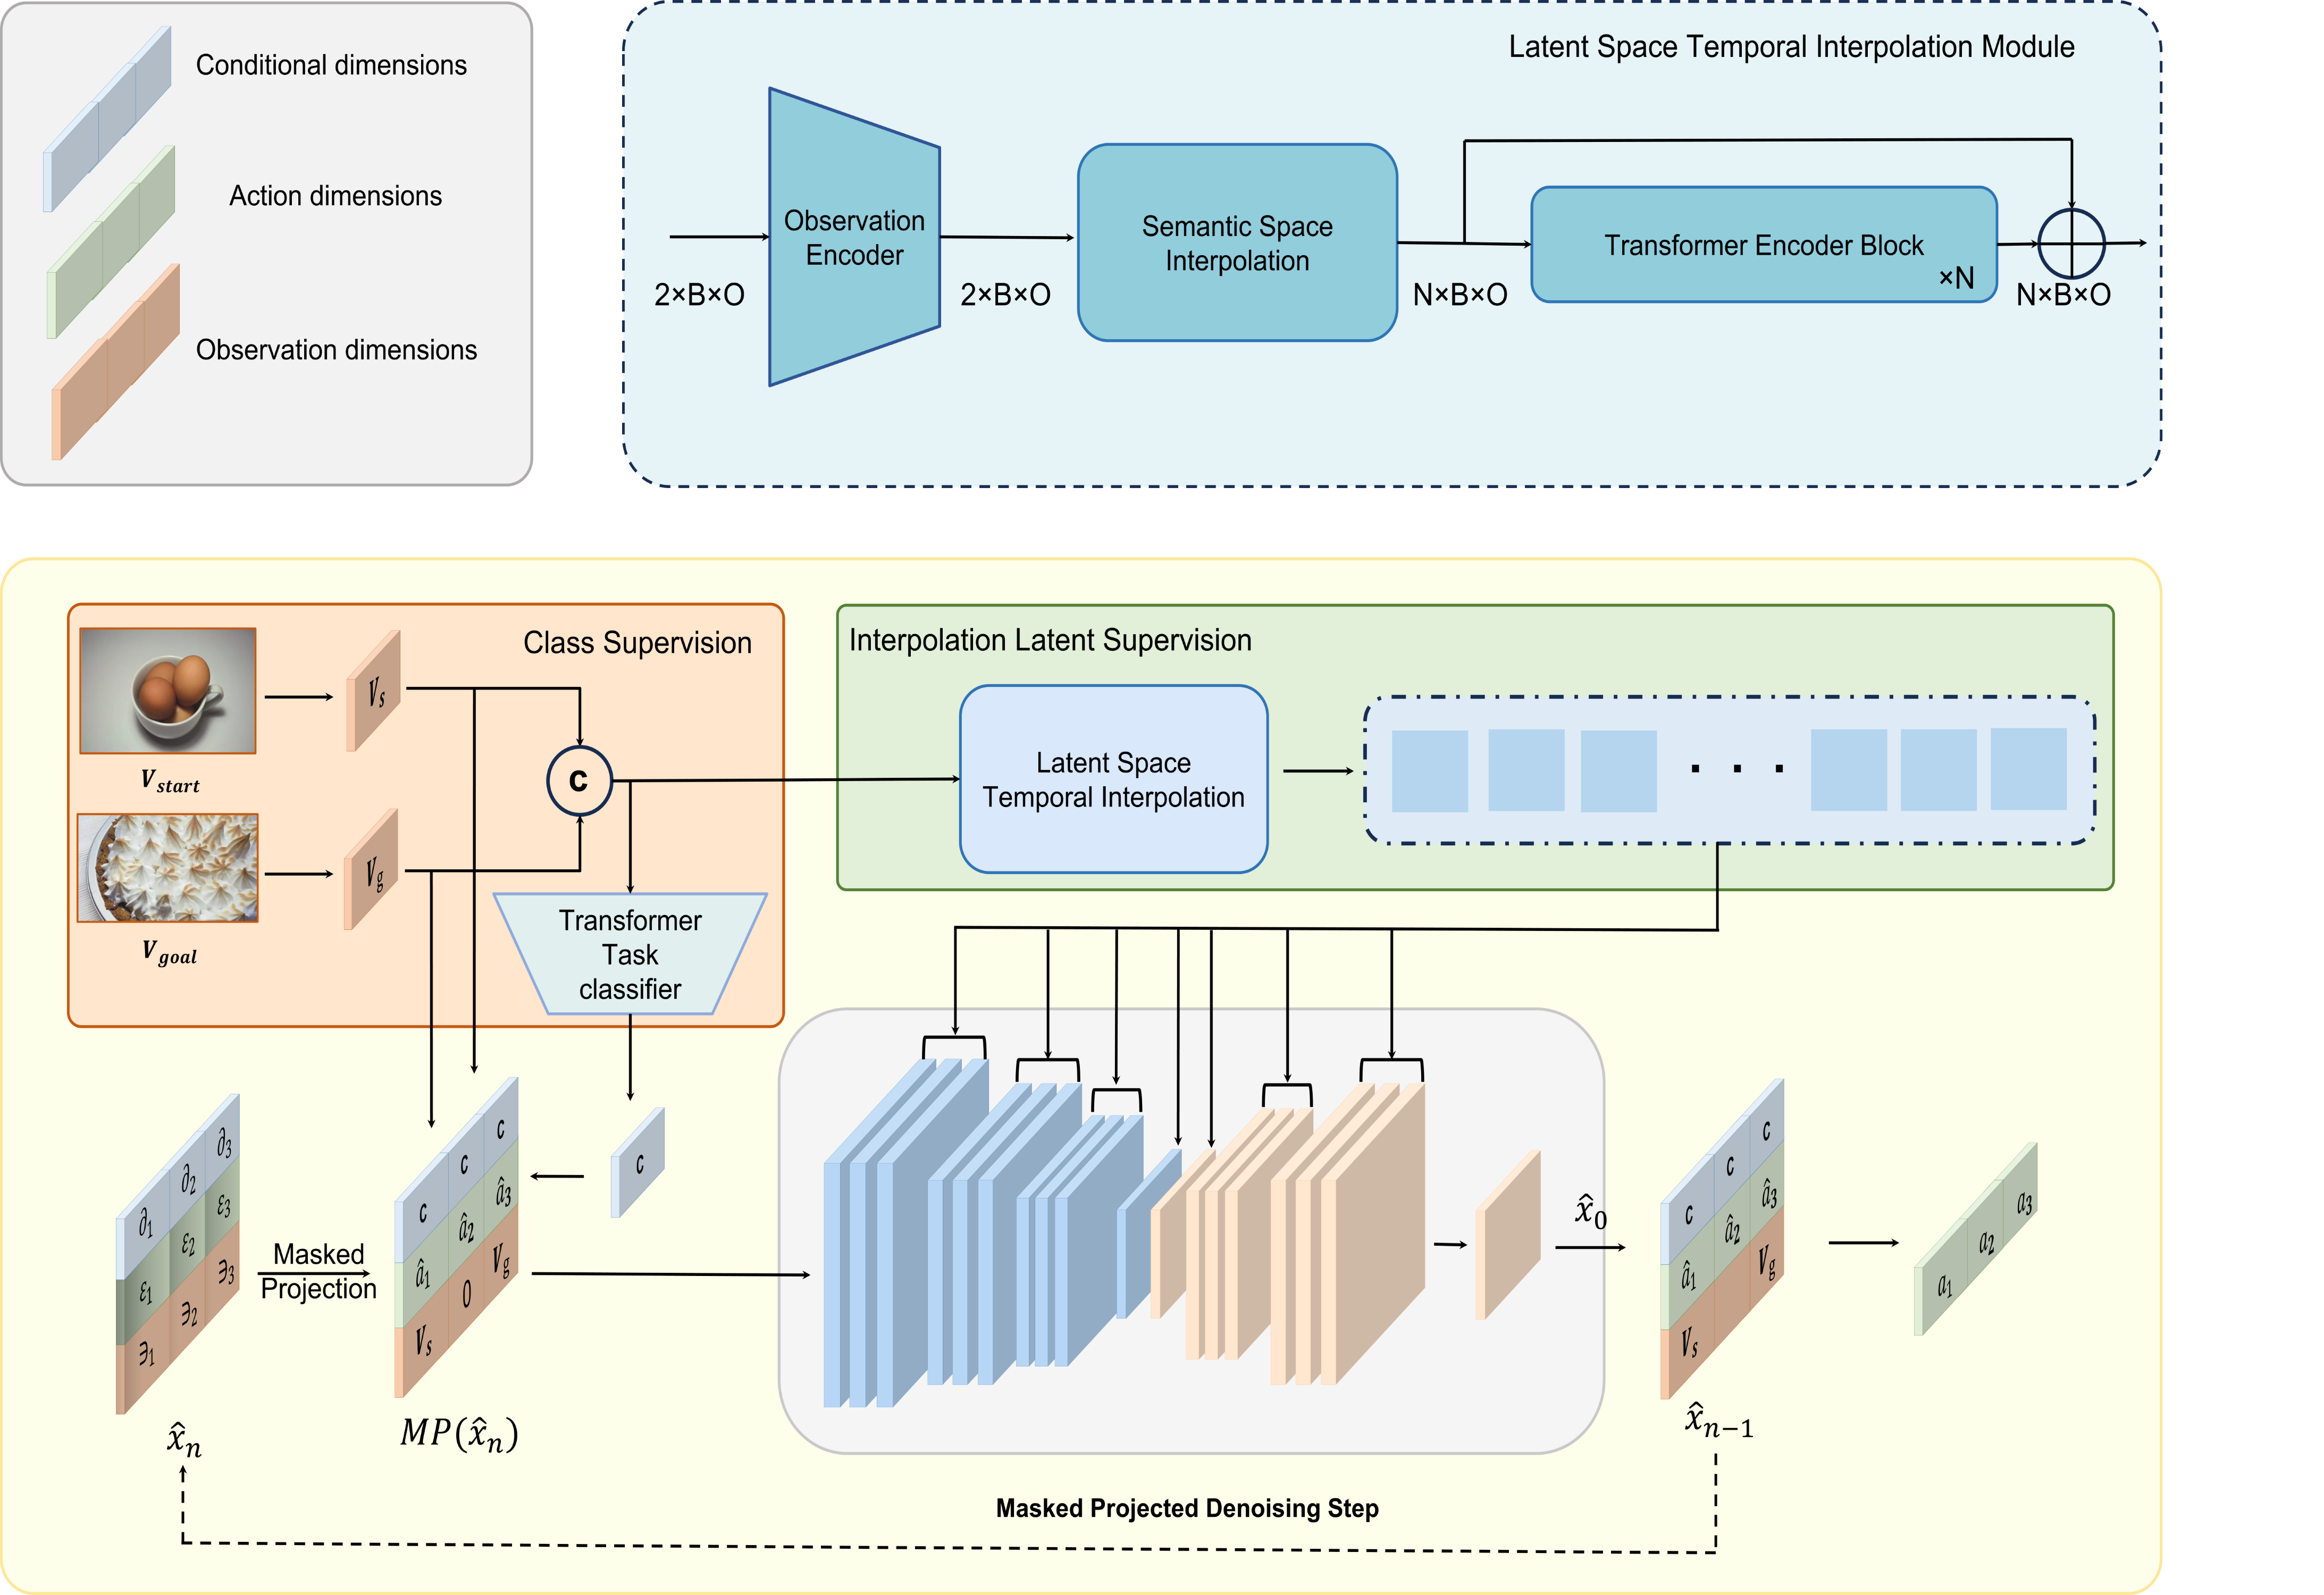
\includegraphics[width=1.06\textwidth, height=0.39\textheight]{figures/architecture.png}
% \hspace{1em} % 增加右方空白
% \vspace{-0.5em} % 增加下方空白
\caption{Overview of our masked temporal interpolation diffusion (prediction horizon $T=3$). We first train a transformer task classifier to generate condition information $c$, which will be used as guidance along with the given observations $V_s$ and $V_g$. Sequentially, we put the concatenated observations into latent space temporal interpolation module to obtain the latent temporal and logic supervision. Then we compute the denoising process iteratively. In each step, we first conduct a masked projection to the input, then predict the initial distribution by the learned model $f(\theta)$. After that we calculate $\hat{x}_{n-1}$ with the U-Net output $\hat{x}_0$. We finally select the action dimensions as our result after $N$ denoising steps. }
\label{fig:architecture}
\end{figure}